\documentclass{article}

% TAE (Trust-AI-Eval) @ NeurIPS 2026 workshop submission — DOUBLE-BLIND, non-archival, <= 8 pages.
% Requires neurips_2026.sty (NeurIPS 2026 template; available on Overleaf as "NeurIPS 2026" or from the
% workshop). The dblblindworkshop option anonymises the author block automatically.
\usepackage[dblblindworkshop]{neurips_2026}

\usepackage{amsmath,amssymb}
\usepackage{booktabs}
\usepackage{graphicx}
\usepackage{microtype}
\usepackage{pgfplots}
\pgfplotsset{compat=1.18}
\usepackage{url}
\usepackage[hidelinks]{hyperref}
\emergencystretch=3em
\Urlmuskip=0mu plus 1mu\relax
\sloppy

\title{How Much of a Leaderboard Ranking Survives Its Own Sampling Error?\\
A Paired-Resolution Audit of Five AI Benchmarks}
\workshoptitle{TAE (Trust-AI-Eval): Can We Trust AI Evaluation?}

% Author block is anonymised by the dblblindworkshop option; do not add names or affiliations.

\begin{document}
\maketitle

\begin{abstract}
A benchmark leaderboard is read as a stopwatch: the rank beside a model is treated as a fact.
Yet every entrant is scored on the \emph{same} items and publishes which it solved, so a
leaderboard is a paired experiment, and its ordering can be tested rather than trusted. We test
each adjacent-rank pair for statistical separability---exact McNemar's test on discordant items for
pass/fail benchmarks, a paired item-bootstrap for scored ones---across five public boards.
On SWE-bench Verified, $129$ of $133$ adjacent ranks are not separable at the $5\%$ level; on MTEB,
$176$ of $180$; on HELM Lite, all $89$ of $89$. The benchmarks are not broken: $88\%$ of \emph{all}
pairs separate cleanly. It is the neighbours they cannot order, and neighbours are what the top of a
table is made of. We derive a resolution bound, $\delta \ge 2.80\sqrt{d/n}$ in the discordance rate
$d$, that predicts which pairs are decidable from a benchmark's size, validate it on $12{,}739$ pairs
with zero false positives, and use LMArena---which already ships confidence intervals and ties---as a
positive control for what correct reporting looks like. Every figure is recomputed from public data
and passes a self-test suite; the recomputed rates match each official board exactly. We argue that a
board should report the \emph{resolution} of its ranking alongside the ranking, at no additional data
cost.
\end{abstract}

\section{Introduction}
Leaderboards have become the primary product of a benchmark: what practitioners take away is not an
evaluation but an \emph{ordering} \citep{hardt2025}. A crisp number sits beside each model and the
order is read as settled. But at the crowded top of a board that order is often softer---an accident
of which items happened to be on the test.

This is checkable, because a benchmark scores every entrant on the same items and (for the boards we
study) each entrant publishes exactly which items it solved. The ordering is therefore a
\emph{paired} experiment: to ask whether model $A$ truly outranks the model directly below it, one
need only look at the items on which they \emph{disagree}. Items both solved, or both missed, carry
no information about the order.

Recent work circles this point from several sides. \citet{singh2025} show that dropping a small share
of Chatbot Arena's data reshuffles its top ranks; \citet{huang2025} reach the same conclusion via
influence functions; \citet{mizzaro2025} find that leaderboard \emph{rankings} stay stable under
paraphrase even as absolute scores collapse; \citet{miller2024} argues for error bars on eval
numbers; and \citet{polo2024} and \citet{kipnis2024} show, through item-response theory, how few items
carry a benchmark's signal. We contribute a direct, uniform, and reproducible test of the object those
threads all bear on---the \emph{rank}---and a bound that says, from a board's size alone, which ranks
it can and cannot resolve. Our contributions:
\begin{enumerate}\itemsep1pt
  \item A single method---exact McNemar for pass/fail, paired item-bootstrap for scores---that tests
  adjacent-rank separability on any board publishing per-item results, applied uniformly to five.
  \item A measured census: most adjacent ranks on four of the five boards are not separable, while
  distant systems separate cleanly, isolating \emph{sampling}, not benchmark quality, as the cause.
  \item A resolution bound $\delta \ge 2.80\sqrt{d/n}$, derived from test power and validated on
  $12{,}739$ pairs with zero false positives, giving the items required to resolve a given gap.
  \item LMArena as a positive control: a board whose confidence intervals and tie-aware ranks already
  report what the others omit, showing the fix is cheap and adopted.
\end{enumerate}

\section{Method}
\label{sec:method}
Let a board rank $m$ systems on $n$ shared items. For a pair $(A,B)$ adjacent in the published order:

\paragraph{Pass/fail benchmarks.} Each item is solved or not. Restricting to the $b+c$ \emph{discordant}
items ($A$ solves and $B$ does not: $b$; the reverse: $c$), the null ``no difference'' is a fair coin,
and we apply the \emph{exact} McNemar test---a two-sided binomial test of $b$ successes in $b+c$ trials
against $p=\tfrac12$. Concordant items cannot distinguish the two systems and are excluded.

\paragraph{Scored benchmarks.} Each item yields a real score per system. We take a paired bootstrap
over items: resample the $n$ items with replacement, recompute each system's mean, and read the $95\%$
interval of the paired difference $A-B$; the pair is separated iff that interval excludes zero. The
same resampled items are used for both systems, preserving the pairing.

\paragraph{Aggregate metrics.} When a board ranks by a composite (e.g.\ a mean win rate over
sub-benchmarks), we first \emph{reproduce the published metric} from raw sub-scores and gate on exact
parity before testing, so we test the number the board actually shows.

\paragraph{Self-tests.} No number is reported before a control suite passes: (i) identical systems are
never ordered, in both modes---the negative control; (ii) $60$ planted losses and a uniform score
shift are both detected at $p<10^{-6}$, so the negative control is not passing merely because nothing
is ever detected; (iii) a published Wilson interval is reproduced ($5/10 \to [0.2366, 0.7634]$).

\section{Results}
\label{sec:results}
On \textbf{SWE-bench Verified} ($134$ systems, $500$ instances), $129$ of the $133$ adjacent-rank pairs
are not separable at $5\%$; eight systems are statistically indistinguishable from the \#1 (ranks
1--8, $76.4$--$79.2\%$); the \#1 and \#2 resolve the same count, and of their $36$ disagreements the
split is $18/18$ ($p=1.000$). Yet $7{,}835$ of all $8{,}911$ pairs ($87.9\%$) \emph{are} separated: the
board discriminates distant systems well. The median $95\%$ rank interval is $13$ places wide of $134$;
$102$ systems span $\ge 10$ places. The recomputed resolve rates match the official board for all $133$
systems with a result file (max $|\Delta|=0$).

Extending to all four SWE-bench splits (Table~\ref{tab:splits}) separates cause from artifact. The
full-size \textbf{Test} split ($2{,}294$ items) has a clear, stable \#1 that survives a $50$-way task
reshuffle every time; the crowded \textbf{Verified}, \textbf{Lite}, and \textbf{Multimodal} splits do
not. A preregistered prediction---that the undecidable gap scales as $1/\sqrt{n}$ from the Verified
anchor---held for $2$ of $3$ held-out splits (the miss, Multimodal, is explained post hoc by its small
pair count and is reported as a miss).

Two further boards, with no shared data, scoring, maintainers, or outcome type, give the same shape.
On \textbf{MTEB} (eng, v2; $181$ systems $\times$ $41$ tasks, scored), $176$ of $180$ adjacent pairs
are not ordered and four systems are tied with the top. On \textbf{HELM Lite} ($90$ models $\times$
$10$ scenarios, ranked by mean win rate) the win-rate matrix reproduces the published index exactly
(max $|\Delta| = 0.0000$) and then \emph{all} $89$ of $89$ adjacent pairs are not separable---the
extreme case, because ten scenarios cannot order ninety models.

\begin{table}[t]
\centering\small
\begin{tabular}{lrrcr}
\toprule
Board & Systems & Items & Adjacent pairs \emph{not} separable & All pairs separated\\
\midrule
SWE-bench Verified & $134$ & $500$ & $129/133$ & $87.9\%$\\
MTEB (eng, v2)     & $181$ & $41$  & $176/180$ & $85.4\%$\\
HELM Lite          & $90$  & $10$  & $\mathbf{89/89}$ & $70.3\%$\\
\midrule
LMArena \emph{(positive control)} & $242$ & 3.5M votes & $238/241$ CIs overlap & ---\\
\bottomrule
\end{tabular}
\caption{Adjacent-rank separability across boards. Distant systems separate ($70$--$88\%$ of all
pairs); neighbours do not. LMArena already reports this via confidence intervals and tie-aware ranks.}
\label{tab:main}
\end{table}

\begin{table}[t]
\centering\small
\begin{tabular}{lrrccr}
\toprule
Split & Systems & Items & Adjacent unclear & \#1 survives reshuffle & Largest unclear gap\\
\midrule
SWE-bench Test        & $24$  & $2{,}294$ & $9/23$  & every time & $1.61$ pp\\
SWE-bench Verified    & $134$ & $500$     & $129/133$ & never    & $4.60$ pp\\
SWE-bench Lite        & $84$  & $300$     & $82/83$ & never      & $6.67$ pp\\
SWE-bench Multimodal  & $12$  & $517$     & $11/11$ & never      & $2.71$ pp\\
\bottomrule
\end{tabular}
\caption{The same test across four SWE-bench splits. Only the large Test split resolves a champion;
the undecidable gap shrinks with $n$, as the preregistered $1/\sqrt{n}$ prediction anticipated.}
\label{tab:splits}
\end{table}

\section{A Resolution Bound}
\label{sec:law}
The pairwise result is not ad hoc. Exact McNemar tests $b/(b+c)$ against $\tfrac12$, and with a gap
$\delta$ in resolve rate and a discordance rate $d$ (the fraction of items on which two systems
differ), $b/(b+c)-\tfrac12 = \delta/2d$. The power of the underlying binomial test then gives
\begin{equation}
\delta \;\ge\; (z_{\alpha/2}+z_{\beta})\,\sqrt{d/n} \;\approx\; 2.80\,\sqrt{d/n}
\qquad (\alpha=0.05,\ \text{power }0.8).
\label{eq:law}
\end{equation}
Two consequences: resolution improves only as $\sqrt{n}$, and---less obviously---it \emph{worsens} as
$\sqrt{d}$: the more two systems differ item-by-item, the harder they are to order at the same headline
gap. Both $d$ and $\delta$ are readable from published files, and no board reports either
(Figure~\ref{fig:frontier}).

\begin{figure}[t]
\centering
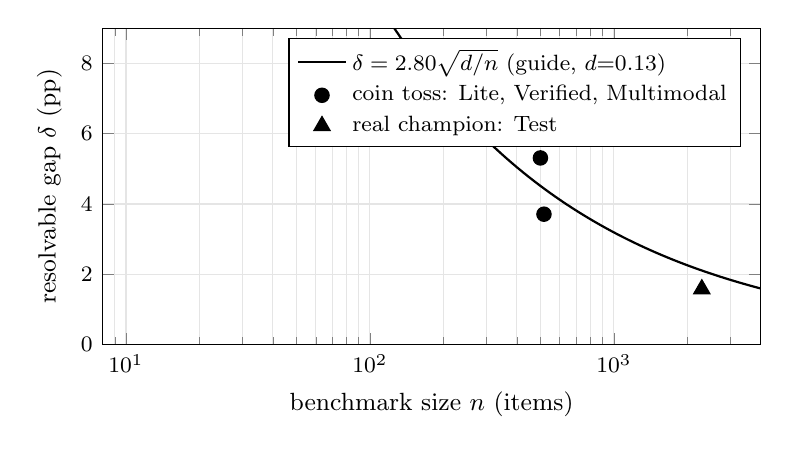
\begin{tikzpicture}
\begin{axis}[
  width=0.82\linewidth, height=5.6cm,
  xmode=log, log basis x=10,
  xlabel={benchmark size $n$ (items)},
  ylabel={resolvable gap $\delta$ (pp)},
  xmin=8, xmax=4000, ymin=0, ymax=9,
  grid=both, grid style={gray!20},
  legend pos=north east, legend cell align=left, legend style={font=\footnotesize},
  tick label style={font=\footnotesize}, label style={font=\small},
]
\addplot[thick, domain=8:4000, samples=120]{2.80*sqrt(0.13/x)*100};
\addlegendentry{$\delta=2.80\sqrt{d/n}$ (guide, $d{=}0.13$)}
\addplot[only marks, mark=*, mark size=2.6pt] coordinates {(300,7.08) (500,5.31) (517,3.71)};
\addlegendentry{coin toss: Lite, Verified, Multimodal}
\addplot[only marks, mark=triangle*, mark size=3.4pt] coordinates {(2294,1.58)};
\addlegendentry{real champion: Test}
\end{axis}
\end{tikzpicture}
\caption{The resolution frontier: the smallest rank gap a benchmark of $n$ items can decide. Each
SWE-bench split is plotted at its own measured near-pair discordance $d$. The three small splits
resolve only $3.7$--$7.1$ pp---coarser than the gaps at their crowded tops---so their neighbours are
ties; only the $2{,}294$-item Test split resolves finely enough ($1.6$ pp) to order a champion.
Resolution improves as $\sqrt{n}$, so a board buys ordering power only by growing.}
\label{fig:frontier}
\end{figure}

We validate Eq.~\eqref{eq:law} pair by pair, predicting each pair's outcome from its own $(\delta,d,n)$
with no free parameters and scoring against the exact test: agreement is $95.6\%$, $92.4\%$, $98.2\%$,
and $89.4\%$ across the four splits, with \textbf{zero false positives} over $12{,}739$ pairs---every
disagreement is a false negative, exactly what an $80\%$-power threshold produces. The bound is thus a
\emph{conservative} certificate: if a gap clears it, the order is real. Priced in items, resolving a
$1$-percentage-point gap on Verified's near-pair discordance would take $\approx 14{,}000$ instances;
the board has $500$, which is why the top eight are one block.

\section{A Positive Control}
\label{sec:lmarena}
LMArena is the board that already does this. It ranks on a Bradley--Terry score with bootstrap $95\%$
confidence intervals, and its published tie-aware rank assigns the \emph{same} rank to models whose
intervals overlap. From its own public numbers ($242$ models), $238$ of $241$ adjacent-by-rating pairs
have overlapping intervals and ranks $2$--$11$ are a ten-way tie---yet the \#1 is genuinely separated,
and the rank column is honest because it surfaces the ties rather than printing a false
$1$-through-$242$ order. This is precisely the change the other four boards need, and it costs a board
nothing it does not already compute.

\section{Discussion}
None of this says the benchmarks are broken; distant systems separate cleanly on every board. It says
a rank is a statistic with a spread, the spread is currently invisible, and readers treat rank $3$ and
rank $7$ as a difference when, for these boards, they usually are not. The remedy is free and the data
already published: where a crowded board prints a lone \#1, show the group statistically tied for
first, or a plausible interval per rank. It makes the false orderings honest and---as LMArena
shows---makes a real champion look exactly as strong as it is. We recommend that leaderboards report
the \emph{resolution} of a ranking, computed from Eq.~\eqref{eq:law} or a paired test, next to the
ranking itself.

\paragraph{Limitations.} The test conditions on the items a board publishes and treats them as the
sampling unit; it measures separability \emph{given} those items and their labels. It does not address
label noise or rater disagreement, a complementary source of rank uncertainty \citep{aroyo2015}, nor
item-selection bias, and it assumes items are exchangeable within a board. These narrow, rather than
overturn, the claim: even granting the labels and the item set, most adjacent ranks are already inside
the sampling noise, so the two uncertainties compound rather than cancel.

\paragraph{Reproducibility.} All data are public; every figure recomputes from a public repository
(anonymised for review; the URL will be included in the camera-ready) that ships the tool, the per-item
matrices, and the self-test suite. The preregistered split prediction was written before the held-out
splits were fetched.

\begin{thebibliography}{9}\small
\bibitem[Hardt(2025)]{hardt2025} M.~Hardt. \emph{The Emerging Science of Machine Learning Benchmarks}. 2025.
\bibitem[Singh et al.(2025)]{singh2025} S.~Singh et al. The Leaderboard Illusion. \emph{arXiv:2504.20879}, 2025.
\bibitem[Huang et al.(2025)]{huang2025} J.~Y.~Huang et al. Dropping Just a Handful of Preferences Can Change Top LLM Rankings. \emph{arXiv:2508.11847}, 2025.
\bibitem[Mizzaro \& Roitero(2025)]{mizzaro2025} S.~Mizzaro and K.~Roitero. On Robustness and Reliability of Benchmark-Based Evaluation of LLMs. 2025.
\bibitem[Miller(2024)]{miller2024} E.~Miller. Adding Error Bars to Evals. \emph{arXiv:2411.00640}, 2024.
\bibitem[Polo et al.(2024)]{polo2024} F.~Maia Polo et al. tinyBenchmarks: Evaluating LLMs with Fewer Examples. \emph{arXiv:2402.14992}, 2024.
\bibitem[Kipnis et al.(2024)]{kipnis2024} A.~Kipnis et al. metabench: A Sparse Benchmark of Reasoning and Knowledge in LLMs. \emph{arXiv:2407.12844}, 2024.
\bibitem[Aroyo \& Welty(2015)]{aroyo2015} L.~Aroyo and C.~Welty. Truth Is a Lie: Crowd Truth and the Seven Myths of Human Annotation. \emph{AI Magazine}, 2015.
\bibitem[Chiang et al.(2024)]{chiang2024} W.-L.~Chiang et al. Chatbot Arena: An Open Platform for Evaluating LLMs by Human Preference. \emph{ICML}, 2024.
\bibitem[Jimenez et al.(2024)]{swebench} C.~E.~Jimenez et al. SWE-bench: Can Language Models Resolve Real-World GitHub Issues? \emph{ICLR}, 2024.
\end{thebibliography}

\end{document}
